\documentclass[table,serif,mathserif,final]{beamer}
\mode<presentation>{\usetheme{Lankton}}
\RequirePackage{ragged2e}
\usepackage{amsmath,amsfonts,amssymb,pxfonts,xspace}
\usepackage{graphicx}
\graphicspath{{./figures/}}
\usepackage[orientation=landscape,size=custom,width=59,height=121,scale=.4,debug]{beamerposter}
%\usepackage{pslatex} % use times roman
\usepackage{amsmath}
\usepackage{amssymb}
\usepackage{amsthm}
\usepackage{color}
\usepackage{array}
\usepackage{xy}
\usepackage{setspace}
\usepackage{tikz}
\usetikzlibrary{matrix}
\usepackage{mathptmx }
\usetikzlibrary{arrows,shapes}
\usepackage{pifont}
\newcommand{\cmark}{{\color{blue}\fontsize{65}{60}\selectfont \ding{51}}}%
\newcommand{\xmark}{{\color{red}\fontsize{65}{60}\selectfont \ding{55}}}%
\newcommand{\citefont}[1]{{\huge \textcolor{gray}{#1}}}


\usepackage[makeroom]{cancel}
\usepackage{verbatim}
\usetikzlibrary{arrows,shapes}


\newcommand*\mycirc[1]{%
  \begin{tikzpicture}
    \node[draw,circle,inner sep=1pt] {#1};
  \end{tikzpicture}}

\newcommand\iitem{\item[\begin{Large}$\bullet$\end{Large}]}

\newcommand{\rot}{\operatorname*{rot}}

%\usepackage[pdftex]{graphicx}
%\usepackage[left=1.5in,right=1.5in, top=1.5in,bottom=1.5in,]{geometry}
\newcommand{\edit}[1]{{\color{red}\textbf{#1}}}
\newcommand{\CC}{\mathbb{C}}
\newcommand{\NN}{\mathbb{N}}
\newcommand{\ZZ}{\mathbb{Z}}
\newcommand{\ot}{\otimes}
\newcommand{\sign}{\operatorname{sign}}

%----------------MACROS---------------%
\newtheorem{thm}{Theorem}[section]
\newtheorem{defn}[thm]{Definition}
\newtheorem{lem}[thm]{Lemma}
\newtheorem{prop}[thm]{Proposition}
\newtheorem{clm}[thm]{Claim} 
\newtheorem{cor}[thm]{Corollary}
\newtheorem{conj}[thm]{Conjecture}
\theoremstyle{remark}
\newtheorem{rem}[thm]{Remark}
\newtheorem{ex}[thm]{Example}

\newcommand{\mycenter}[1]{\hfil #1 \hfil}
\newcommand{\myzero}{\hfil $0$ \hfil}
\newcommand{\ca}{\cellcolor{ca}}
\newcommand{\cb}{\cellcolor{cb}}
\newcommand{\cc}{\cellcolor{cc}}
\def \av {\text{AV}}
\newcommand{\match}[3]{
\item {\textbf{#1}\newline Appears for #2 sets of patterns. \\ Example match: $\av_n($#3$)$ }
}
\newcommand{\matchone}[2]{
\item {\textbf{#1}\newline Match: #2 \newline}
}

\newcommand{\footleft}{}
\newcommand{\footright}{}
%% %\dologotrue
\title{Cache Efficient Parallel Partition Algorithms \\An In-Place Exclusive Read/Write Memory Algorithm}

%-- Header and footer information ----------------------------------
\setbeamertemplate{headline}{
 \leavevmode
    \vskip1cm
    \centering
    \usebeamercolor{title in headline}{\fontsize{40}{50}\selectfont \textbf{\inserttitle} \\[0.5ex]}
    % \usebeamercolor{author in headline}{\Huge{\insertauthor}\\[1ex]}
    % \usebeamercolor{institute in headline}{\Huge{\insertinstitute}\\[1ex]}

 \hspace{0.5in}\begin{beamercolorbox}[wd=47in,colsep=0.15cm]{cboxb}\end{beamercolorbox}
}


%-------------------------------------------------------------------
\definecolor{math}{rgb}{0.4,0.4,1}
%\definecolor{proven}{rgb}{0.4,0.4,1}
%\definecolor{conject}{rgb}{0.7.0,7,1}
%\definecolor{comput}{rgb}{09,0.9,1}
%\definecolor{lightslateblue}{rgb}{0.517647,0.43921569,1} % light slate blue 0x8470ff (132,112,255)
%\definecolor{proven}{rgb}{0.52941176,0.80784313,0.98039} % sky blue 0x87ceeb (135,206,250)
%\definecolor{conject}{rgb}{0.7.0,7,1}
%\definecolor{comput}{rgb}{0.9,0.9,1}
%\definecolor{proven}{rgb}{0.7,1,1} % sky blue 0x87ceeb (135,206,250)
%\definecolor{conject}{rgb}{0.4,0.4,1}
%\definecolor{comput}{rgb}{1,0.9,1}

%\definecolor{proven}{rgb}{0.59608,0.98431,0.59608} % pale green 0x98fb98 152,251,152
%\definecolor{comput}{rgb}{0.75,1,0.75} % pale green 0x98fb98 152,251,152
\definecolor{ca}{rgb}{0.875,1,0.875} % lighter than pale green
\definecolor{cb}{rgb}{0.75,1,1} % sky blue 0x87ceeb (135,206,250)
\definecolor{cc}{rgb}{1,0.9,1}
%\definecolor{comput}{rgb}{1,1,1} % sky blue 0x87ceeb (135,206,250)


\definecolor{darkgreen}{rgb}{0.4,0.8,0.5} 

%-- Main Document --------------------------------------------------
\begin{document}
\begin{frame}{}
\begin{columns}[t]
  \begin{column}{0.5\linewidth}
\begin{block}{\Huge Our Research Question}
  \justifying
  \Huge Can we create an algorithm with \emph{theoretical guarantees} that is \emph{fast in practice}?
\end{block}

\begin{block}{\Huge Result}
  \justifying
  \Huge We created the \emph{Smoothed Striding Algorithm}. \\
  Key Features:
	\begin{itemize}
		\item linear work and polylogarithmic span \\
			{\color{blue} (like the Standard Algorithm)\\}
		\vspace{0.15cm}
		\item fast in practice \\
			{\color{blue} (like the Strided Algorithm)\\}
	\vspace{0.15cm}
		\item theoretically optimal cache behavior \\
			{\color{blue} (unlike any past algorithm)}
	\end{itemize}
\end{block}

\begin{block}{\Huge Smoothed Striding Algorithm's Performance}
	\begin{figure}
		\begin{center}
			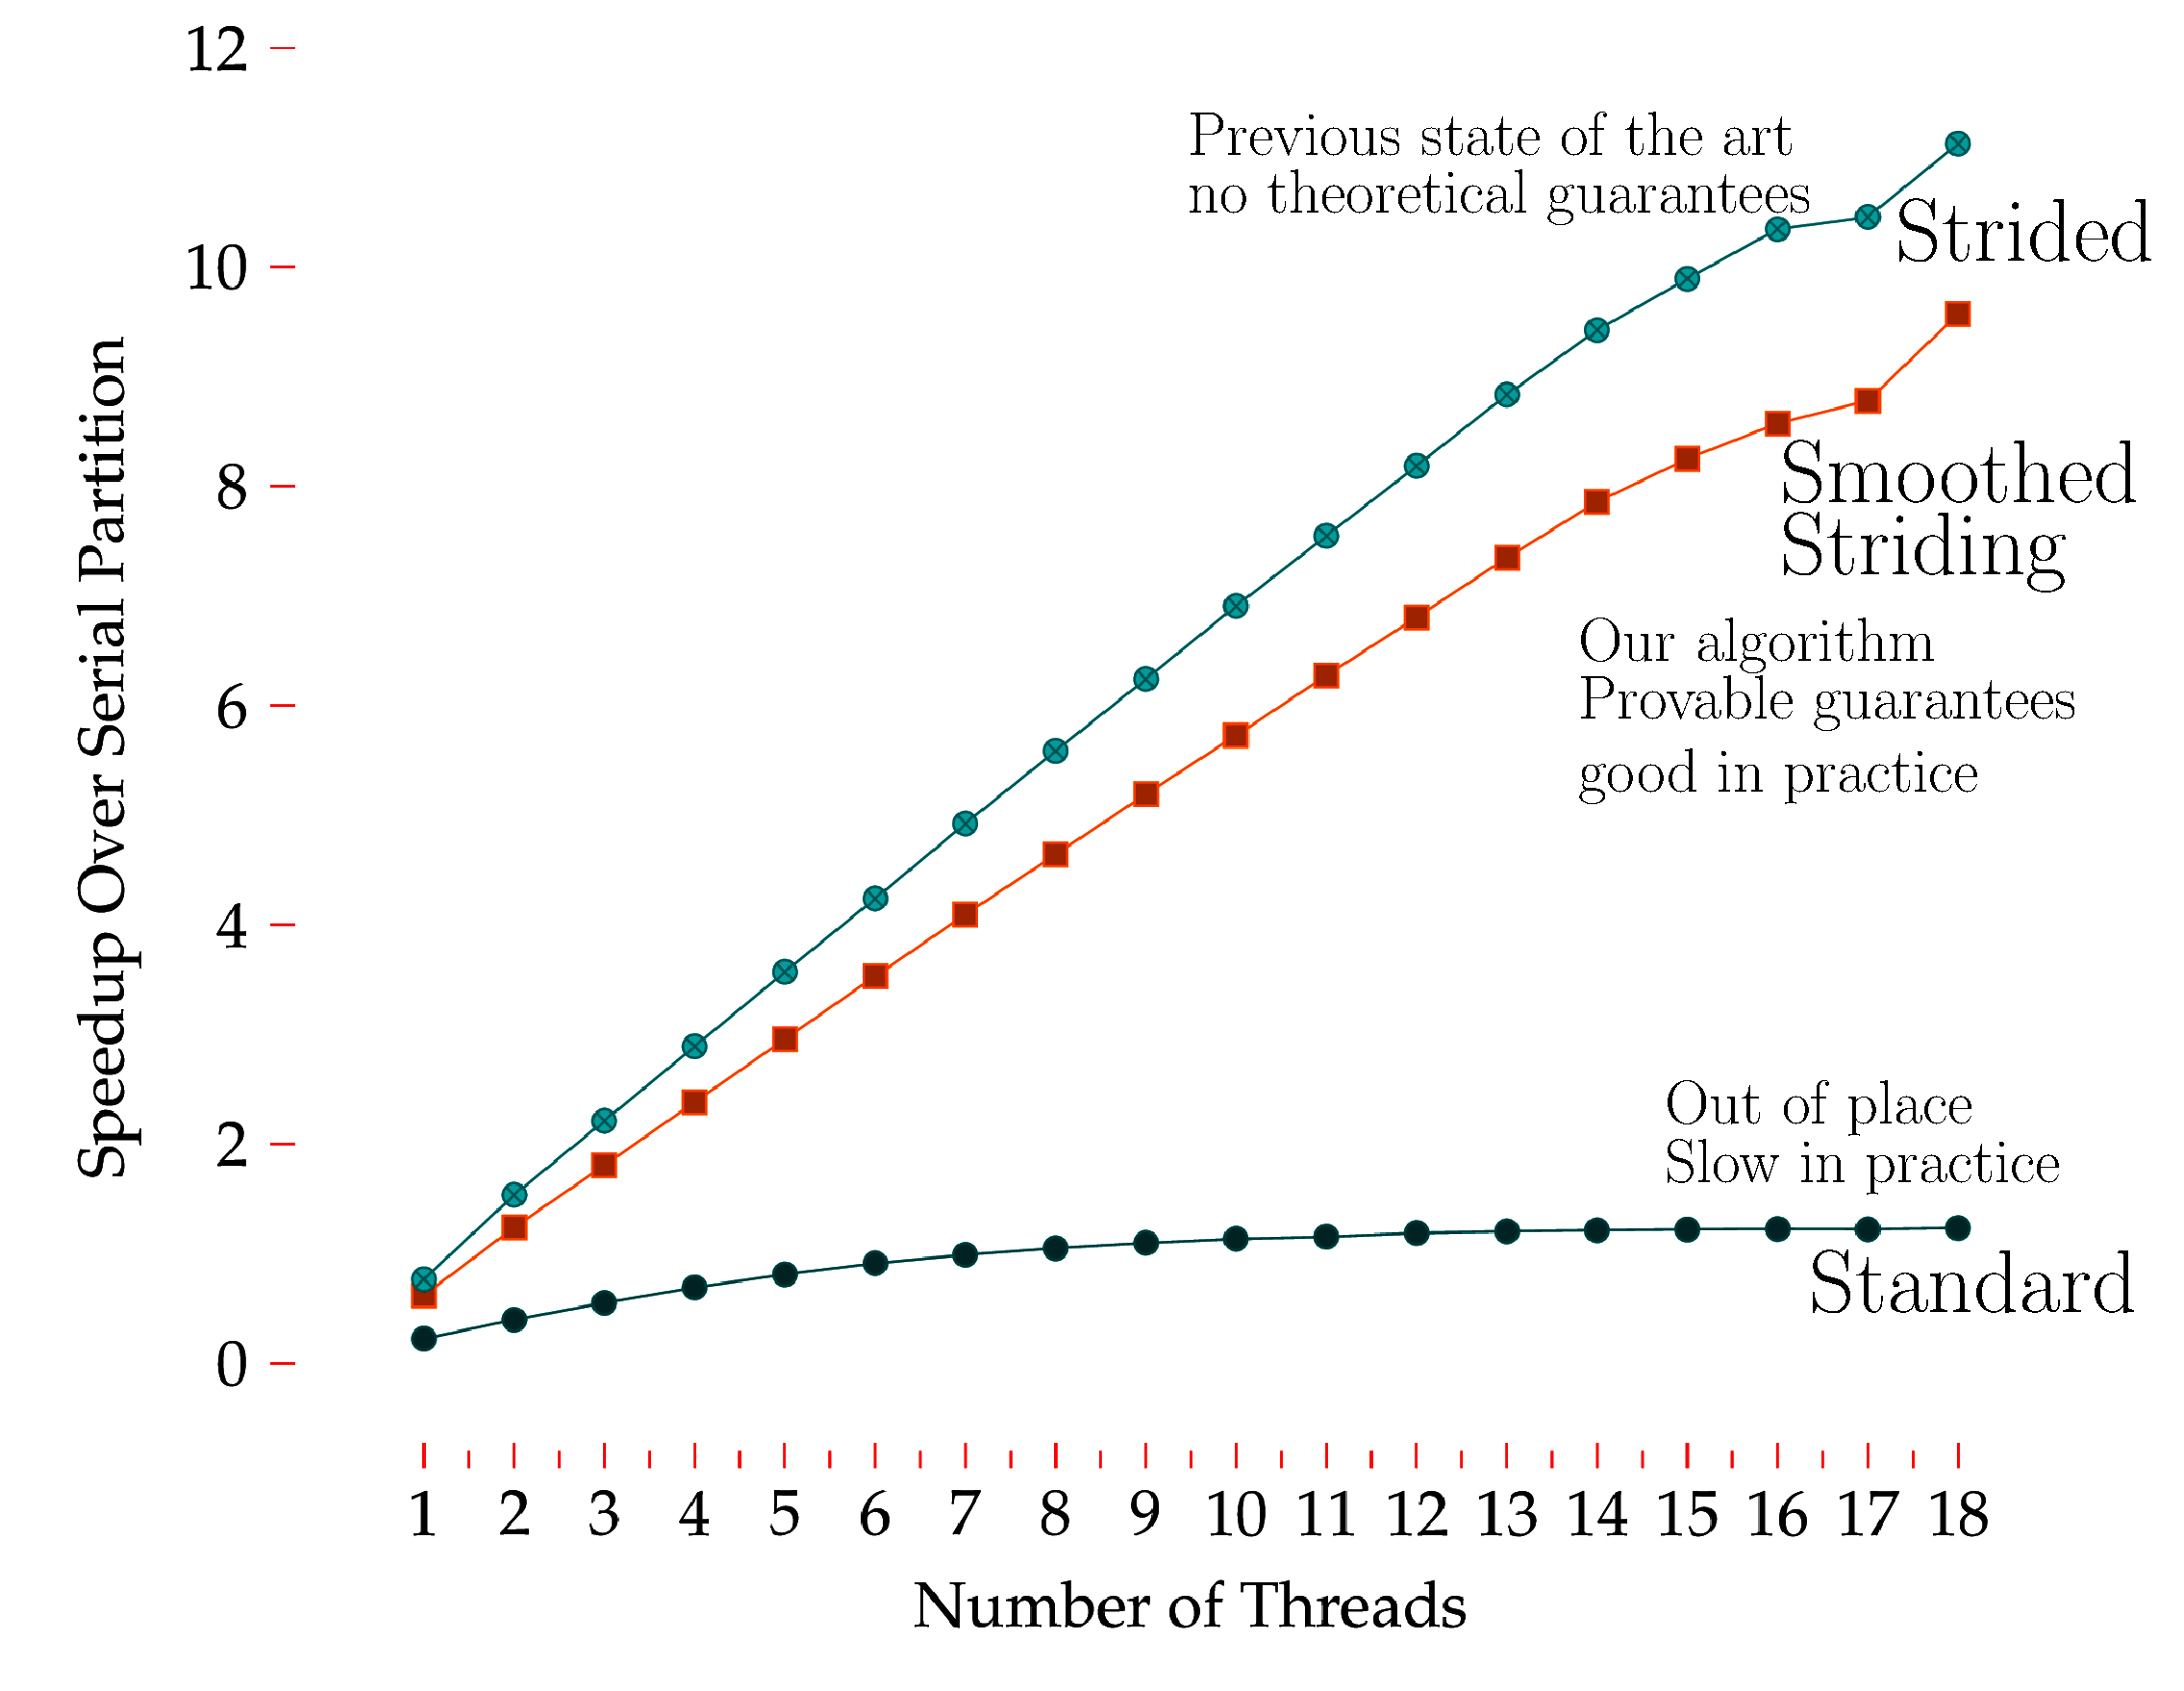
\includegraphics[width=0.9\linewidth]{imgs/compiledGraph.eps}
		\end{center}
	\end{figure}
\end{block}

\begin{block}{\Huge Strided Versus Smoothed-Striding Algorithm}
  \Huge
	\begin{columns}[T] % align columns
	\begin{column}{.45\textwidth}
		\textbf{Strided Algorithm}\\\citefont{[Francis and Pannan, 92; Frias and Petit, 08]}\\
		\vspace{0.25cm}
		\begin{itemize}
			\item Good cache behavior in practice\\\hfill
			\item Worst case span is $T_\infty \approx n$\\\hfill\\\hfill
			\item On random inputs span is $T_\infty = \tilde{O}(n^{2/3})$
		\end{itemize}
	\end{column}
	\hfill
	\begin{column}{.55\textwidth}
		\textbf{Smoothed-Striding Algorithm}\\\citefont{}\\
		\vspace{0.25cm}
		\begin{itemize}
			\item Provably optimal cache behavior\\\hfill
			\item Span is \\$T_\infty = O(\log n \log\log n)$\\ with high probability in $n$\\\hfill
			\item Uses randomization \emph{inside} the algorithm % both about the recursion step and the no worst case inputs thing
		\end{itemize}
	\end{column}
	\end{columns}

\end{block}

  \end{column}

  \begin{column}{0.5\linewidth}
\begin{block}{\Huge Smoothed Striding Algorithm}
  \Huge
	Logically partition the array into chunks of adjacent elements.
	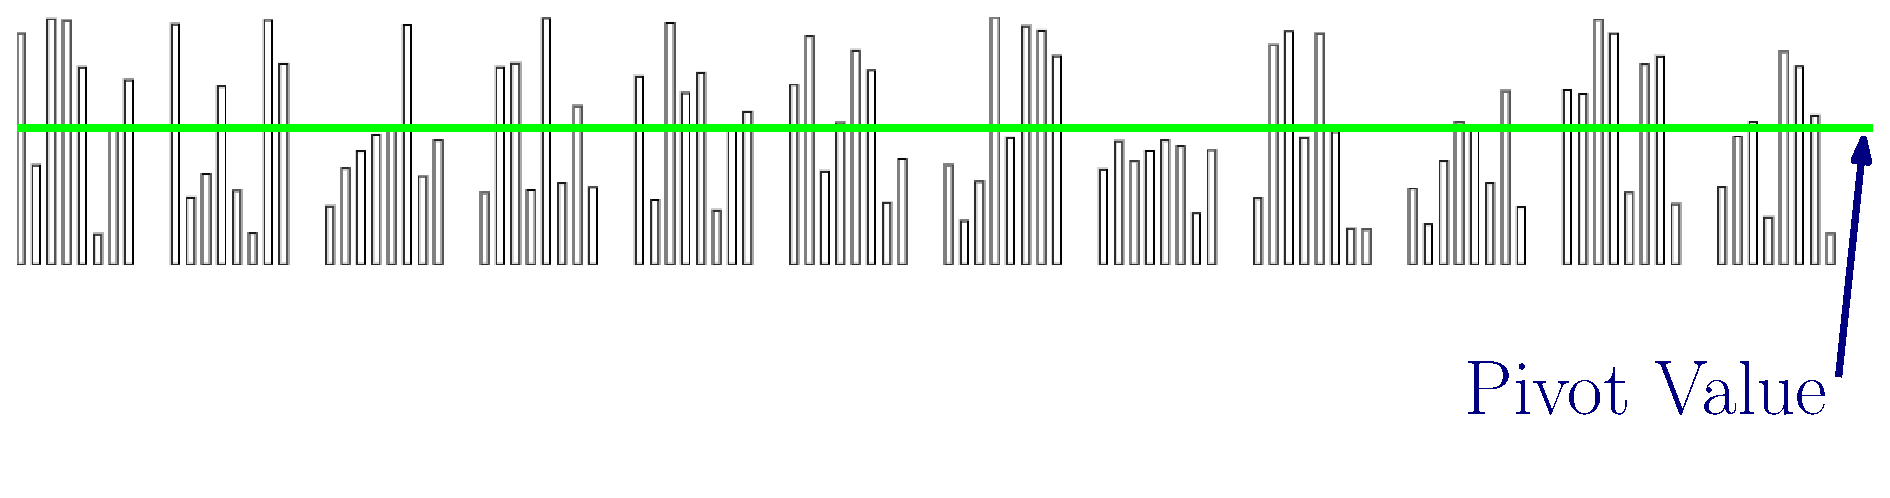
\includegraphics[width=\linewidth]{imgs/smoothedStridingAlgSim/sim1.eps}
	Form groups $U_i$ that contain a random element from each chunk. \\
  {\color{blue}This randomization step was one of our key insights; it guarantees that the $U_i$'s have similar compositions regardless of the input.}
	\includegraphics[width=\linewidth]{imgs/smoothedStridingAlgSim/sim2.eps}
	Perform serial partitions on each $U_i$ in parallel over the $U_i$'s. \\
  This step is highly parallel.
	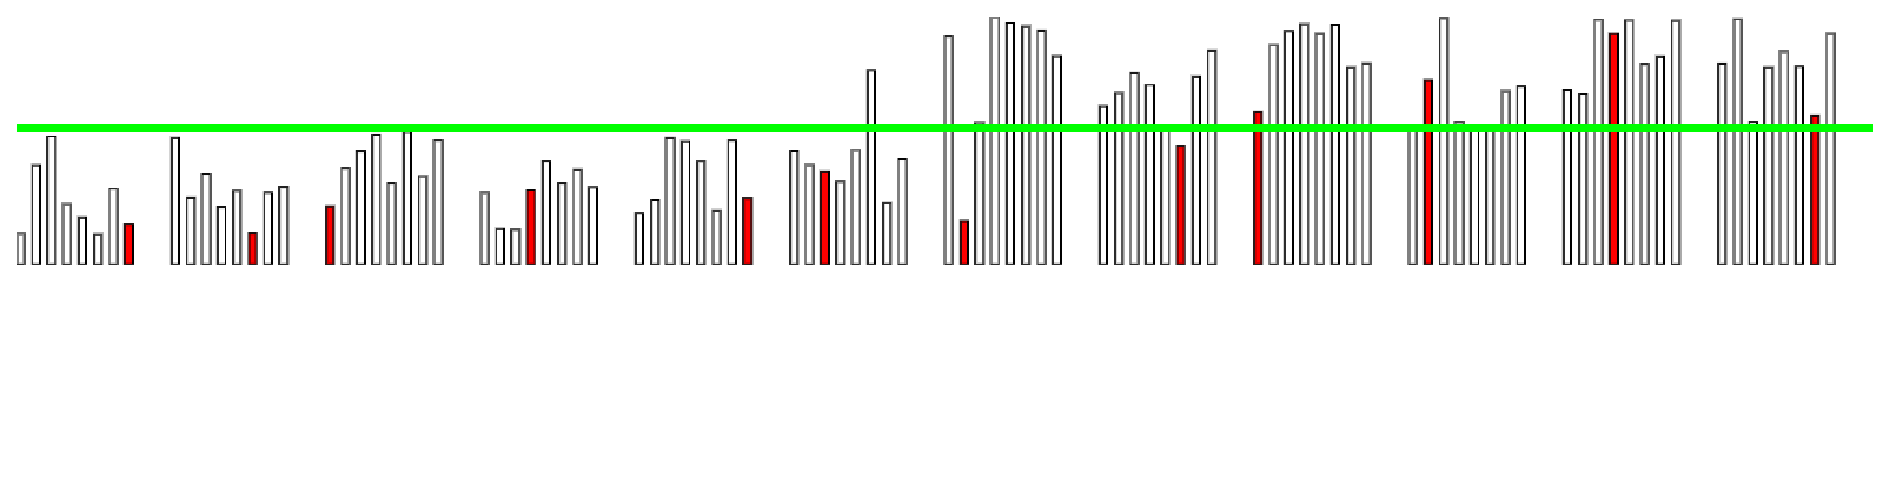
\includegraphics[width=\linewidth]{imgs/smoothedStridingAlgSim/sim3.eps}
  Define $v_i = $ index of first element greater than the pivot in $U_i$. 
	\includegraphics[width=\linewidth]{imgs/smoothedStridingAlgSim/sim35.eps}
  Identify leftmost and rightmost $v_i$. Note that $A[k] \le \text{pivot}$ for all $k < v_{\min}$, and $A[k] > \text{pivot}$ for all $k \ge v_{\max}$.
	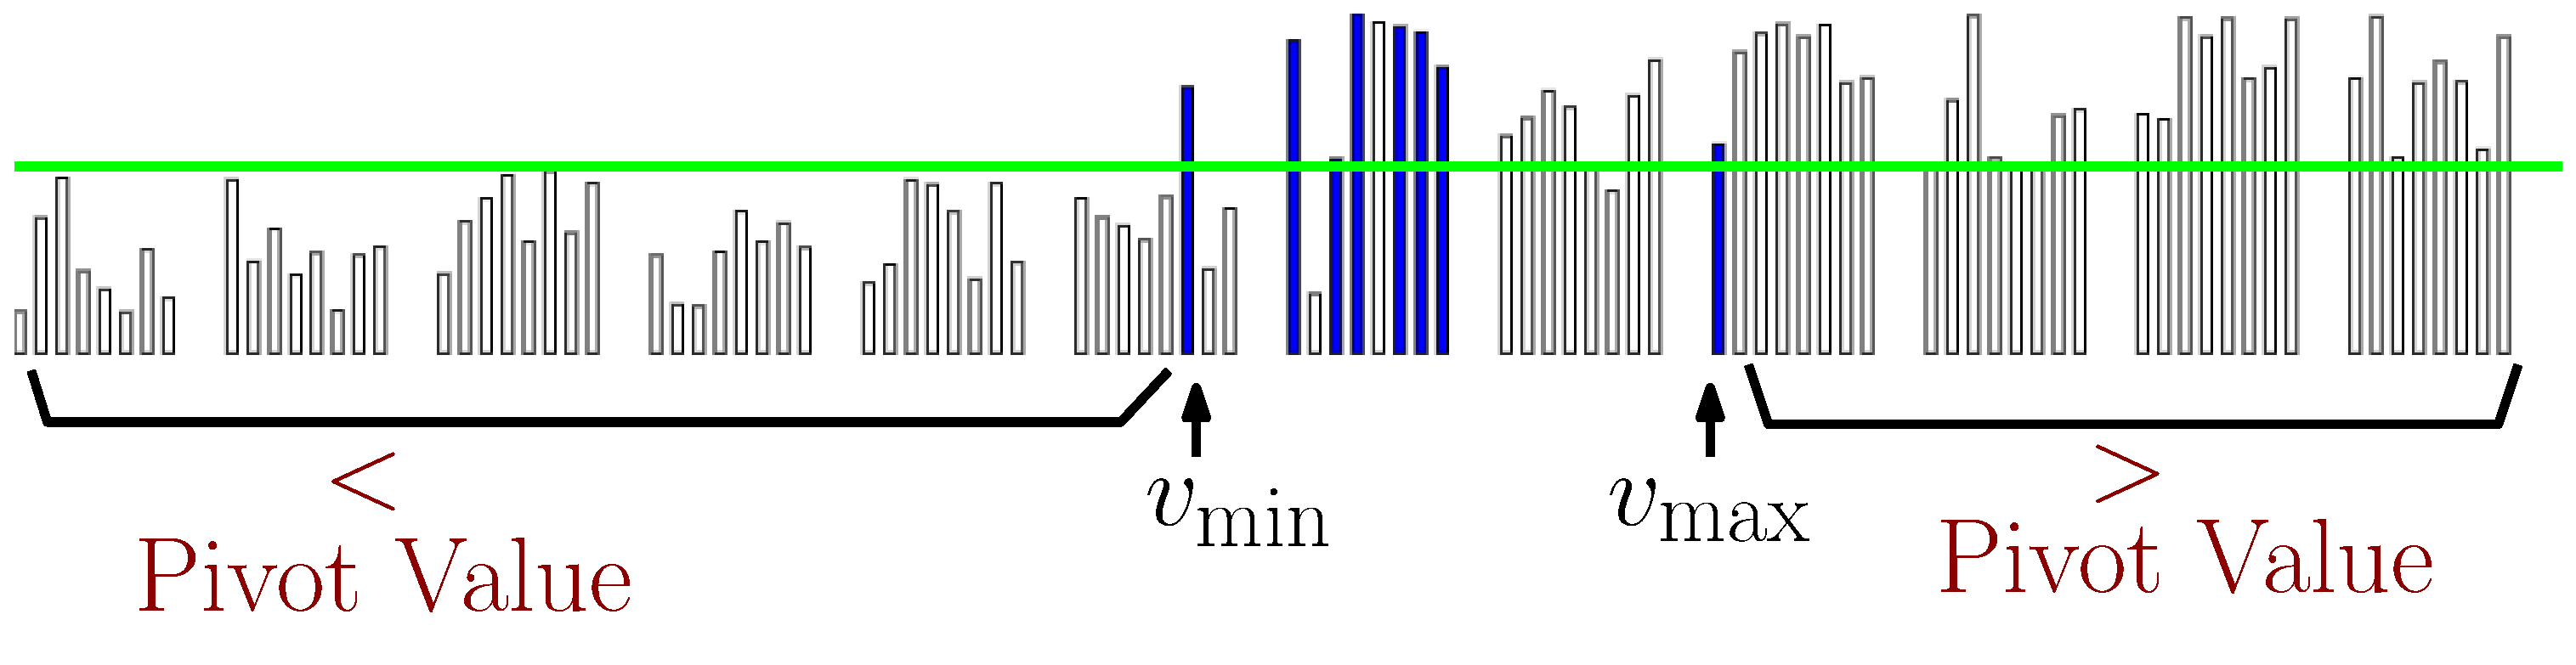
\includegraphics[width=\linewidth]{imgs/smoothedStridingAlgSim/sim4.eps}
	Recursively partition the subarray.\\
  {\color{blue}This step was previously impossible; adding randomization enables this step, which enables our algorithm's low span. }
	\includegraphics[width=\linewidth]{imgs/smoothedStridingAlgSim/sim45.eps}
\end{block}

\begin{block}{\Huge A Key Challenge}
  \Huge
How do we store the $U_i$'s if they are all random?	\\
\vspace{0.5cm}
Storing which elements make up each $U_i$ takes too much space!\\

\vspace{0.5cm}
\textbf{Strided Algorithm $P_i$.}
\begin{figure}
	\includegraphics[width=\linewidth]{imgs/stridedAlgHighlighted.png}
\end{figure}
\textbf{Smoothed-Striding Algorithm $U_i$.}
\begin{figure}
	\includegraphics[width=\linewidth]{imgs/smoothedStridingAlgHighlighted.png}
\end{figure}
\end{block}

\begin{block}{How to Store the groups}
  %TODO fix
  \Huge
	\textbf{Key Insight:} While each $U_i$ does need to contain a random element from each chunk, the $U_i$'s don't need to be \emph{independent}.

	\vspace{0.5cm}
	We store $U_1$, and all other groups are determined by a "circular shift" of $U_1$ (wraparound within each chunk).
	% Specifically, let $X$ be an array with values chosen uniformly from $\{1,2,\ldots,g\}$. Then the $i$-th element of $U_j$ has index 
	% $$ 1 + ((X[i]+j)\mod g)$$
	\vspace{0.5cm}
	\begin{figure}
		\includegraphics[width=\linewidth]{imgs/blackrainbowAlt.eps}
	\end{figure}	
\end{block}
\end{column}

\end{columns}
\end{frame}
\end{document}
